\chapter{Results}
\label{chap:Results}

\indent Unblinded signal region distributions of the kinematic variables with the most discrimination power are shown in Figure \ref{fig:SRCUnblined}.  The expected background yield have been normalized to all control regions using the background only fitting procedure described in section \ref{sec:stat:bkgonly}.  \\

\begin{figure}[!h] 
\begin{center}
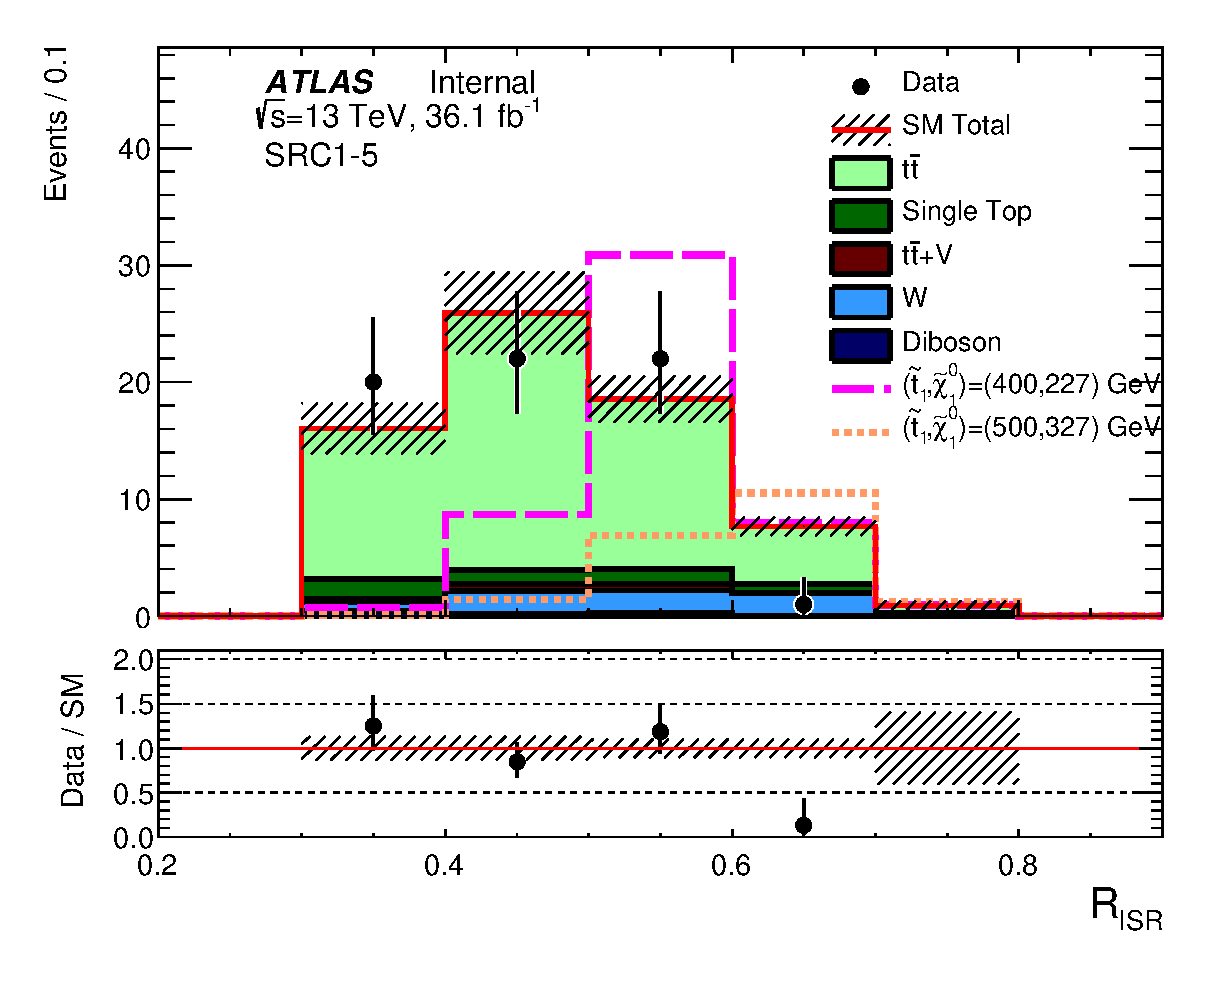
\includegraphics[width=0.85\textwidth]{figures/SRC/CA_RISR_SRC1_5}
%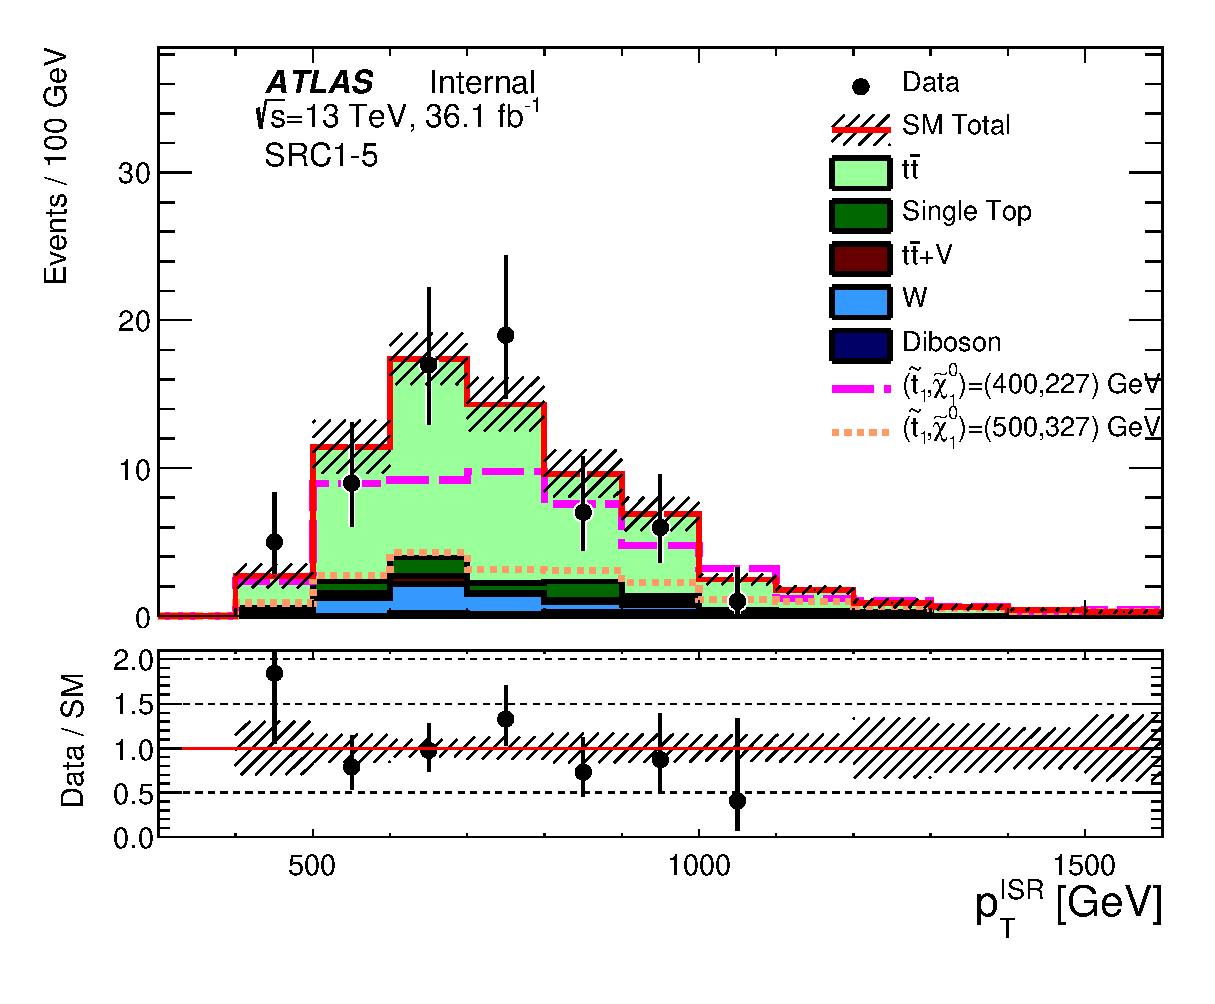
\includegraphics[width=0.45\textwidth]{figures/SRC/CA_PTISR_SRC1_5}
%\caption{Unblinded \rISR\ and \pTISR\ distributions for SRC1-5 for \intlumi\ \ifb.}
\caption{Unblinded $\rISR$  distributions for SRC1-5 for \intlumi\ \ifb.}
\label{fig:SRCUnblined}
\end{center}
\end{figure}

\indent Signal region yields with $\intlumi$ $\ifb$ of data can be seen in Table \ref{table.bkgonly.SRC1to3}.  No significant excess is observed in any region.  An under fluctuation of background is observed in the $\RISR$ bin between $0.6-0.7$ but is not statistically significant due to the low amount of expected events.  \\



\begin{table}[!h]
\begin{center}
\setlength{\tabcolsep}{0.0pc}
{\small
%%
\begin{tabular*}{\textwidth}{@{\extracolsep{\fill}}lrrr}
\noalign{\smallskip}\hline\noalign{\smallskip}
{\bf SRC yields}           & SRC1            & SRC2            & SRC3              \\[-0.05cm]
\noalign{\smallskip}\hline\noalign{\smallskip}
%%
Observed events          & $20$              & $22$              & $22$                    \\
\noalign{\smallskip}\hline\noalign{\smallskip}
%%
Expected bkg events         & $21.02 \pm 6.62$          & $28.42 \pm 4.89$          & $19.60 \pm 3.53$              \\
\noalign{\smallskip}\hline\noalign{\smallskip}
%%
        Expected TTbar events         & $12.85 \pm 5.87$          & $22.05 \pm 4.19$          & $14.57 \pm 3.23$              \\
%%
        Expected Wjets events         & $0.81 \pm 0.37$          & $1.93 \pm 0.48$          & $1.91 \pm 0.63$              \\
%%
        Expected Zjets events         & 0.46 $\pm$ 0.09          & 0.90 $\pm$ 0.13          &  0.74 $\pm$ 0.15               \\
%%
        Expected TtbarV events         & $0.29 \pm 0.18$          & $0.59 \pm 0.38$          & $0.56 \pm 0.31$              \\
%%
        Expected SingleTop events         & $1.67_{-1.67}^{+2.02}$          & $1.18_{-1.18}^{+1.81}$          & $1.22_{-1.22}^{+1.37}$              \\
%%
        Expected Diboson events         & $0.39 \pm 0.33$          & $0.21 \pm 0.11$          & $0.29 \pm 0.18$              \\
%%
        Expected Multijets events         & $4.56 \pm 2.38$          & $1.58 \pm 0.77$          & $0.32 \pm 0.17$              \\
%%     
 \noalign{\smallskip}\hline\noalign{\smallskip}

\end{tabular*}
%%%

\begin{tabular*}{\textwidth}{@{\extracolsep{\fill}}lrr}
\noalign{\smallskip}\hline\noalign{\smallskip}
{\bf SRC yields}           & SRC4            & SRC5              \\[-0.05cm]
\noalign{\smallskip}\hline\noalign{\smallskip}
%%
Observed events          & $1$              & $0$                    \\
\noalign{\smallskip}\hline\noalign{\smallskip}
%%
Expected bkg events         & $8.14 \pm 1.39$          & $0.99 \pm 0.71$              \\
\noalign{\smallskip}\hline\noalign{\smallskip}
%%
        Expected TTbar events         & $4.92 \pm 0.98$          & $0.63_{-0.63}^{+0.69}$              \\
%%
        Expected Wjets events         & $1.93 \pm 0.45$          & $0.21 \pm 0.12$              \\
%%
        Expected Zjets events         & 0.45 $\pm$ 0.24          & 0.09 $\pm$ 0.04             \\
%%
        Expected TtbarV events         & $0.08 \pm 0.08$          & $0.06 \pm 0.03$              \\
%%
        Expected SingleTop events         & $0.72_{-0.72}^{+0.77}$          & $0.00 \pm 0.00$              \\
%%
        Expected Diboson events         & $0.00 \pm 0.00$          & $0.00 \pm 0.00$              \\
%%
        Expected Multijets events         & $0.04 \pm 0.02$          & $0.00 \pm 0.00$              \\
%%     
 \noalign{\smallskip}\hline\noalign{\smallskip}
\end{tabular*}

}
\end{center}
\caption{Region: SRC. Background-only fit results for an integrated luminosity of 36.07 \ifb. The uncertainties are statistical and systematic.
}
\label{table.bkgonly.SRC1to3}
\end{table}
%

%

\begin{table}
\begin{center}
\setlength{\tabcolsep}{0.0pc}
{\small
%%
\begin{tabular*}{\textwidth}{@{\extracolsep{\fill}}lrr}
\noalign{\smallskip}\hline\noalign{\smallskip}
{\bf SRC yields}           & SRC4            & SRC5              \\[-0.05cm]
\noalign{\smallskip}\hline\noalign{\smallskip}
%%
Observed events          & $1$              & $0$                    \\
\noalign{\smallskip}\hline\noalign{\smallskip}
%%
Expected bkg events         & $8.14 \pm 1.39$          & $0.99 \pm 0.71$              \\
\noalign{\smallskip}\hline\noalign{\smallskip}
%%
        Expected TTbar events         & $4.92 \pm 0.98$          & $0.63_{-0.63}^{+0.69}$              \\
%%
        Expected Wjets events         & $1.93 \pm 0.45$          & $0.21 \pm 0.12$              \\
%%
        Expected Zjets events         & 0.45 $\pm$ 0.24          & 0.09 $\pm$ 0.04             \\
%%
        Expected TtbarV events         & $0.08 \pm 0.08$          & $0.06 \pm 0.03$              \\
%%
        Expected SingleTop events         & $0.72_{-0.72}^{+0.77}$          & $0.00 \pm 0.00$              \\
%%
        Expected Diboson events         & $0.00 \pm 0.00$          & $0.00 \pm 0.00$              \\
%%
        Expected Multijets events         & $0.04 \pm 0.02$          & $0.00 \pm 0.00$              \\
%%     
 \noalign{\smallskip}\hline\noalign{\smallskip}
\end{tabular*}
%%%
}
\end{center}
\caption{Region: SRC. Background-only fit results for an integrated luminosity of 36.07 \ifb. The uncertainties are statistical and systematic.
}
\label{table.bkgonly.SRC4to5}
\end{table}
%


\indent 95 percent upper confidence limits on the observed cross-section ($\langle\epsilon\sigma\rangle_{\rm obs}^{95}$) and on the number of signal events ($S_{\rm obs}^{95}$) in each $\RISR$ bin is shown in Table \ref{table.results.exclxsec.pval.upperlimit}.  The observed signal cross-section is defined as the number of signal events predicted to exist in SR for any particular signal model and is equivalent to selection efficiency times the signal production cross-section.  The limit on the observed cross-section is completely theory independent.  It is simply a statement on the maximum additional BSM rate that can exist in the signal region without being ruled out to 95 percent confidence. \\

\indent Observed limits are derived using the discovery fit procedure described in section \ref{sec:stat:discovery}.  Discovery p-values are calculated using the asymptotic high statistics assumption.  \\


\begin{table}[!h]
\centering
\setlength{\tabcolsep}{0.0pc}
\begin{tabular*}{\textwidth}{@{\extracolsep{\fill}}lccccc}
\noalign{\smallskip}\hline\noalign{\smallskip}
{\bf Signal channel}                        & $\langle\epsilon{\rm \sigma}\rangle_{\rm obs}^{95}$[fb]  &  $S_{\rm obs}^{95}$  & $S_{\rm exp}^{95}$ & $CL_{B}$ & $p(s=0)$ ($Z$)  \\
\noalign{\smallskip}\hline\noalign{\smallskip}
%%
SRC1    & $0.44$ &  $16.0$ & $ { 16.3 }^{ +5.8 }_{ -4.2 }$ & $0.47$ &
 $ 0.50$~$(0.00)$ \\%
SRC2    & $0.35$ &  $12.6$ & $ { 15.5 }^{ +5.9 }_{ -4.2 }$ & $0.26$ &
$ 0.50$~$(0.00)$ \\%
SRC3    & $0.44$ &  $15.8$ & $ { 12.8 }^{ +4.7 }_{ -2.7 }$ & $0.69$ &
$ 0.30$~$(0.54)$ \\%
SRC4    & $0.09$ &  $3.1$ & $ { 6.5 }^{ +3.3 }_{ -2.1 }$ & $0.02$ & $
0.50$~$(0.00)$ \\%
SRC5    & $0.06$ &  $2.2$ & $ { 2.8 }^{ +2.0 }_{ -1.1 }$ & $0.32$ & $
0.49$~$(0.02)$ \\%

\noalign{\smallskip}\hline\noalign{\smallskip}
\end{tabular*}
\caption[Breakdown of upper limits.]{
Left to right: 95\% CL upper limits on the visible cross section
($\langle\epsilon\sigma\rangle_{\rm obs}^{95}$) and on the number of
signal events ($S_{\rm obs}^{95}$ ).  The third column
($S_{\rm exp}^{95}$) shows the 95\% CL upper limit on the number of
signal events, given the expected number (and $\pm 1\sigma$
excursions on the expectation) of background events.
The last two columns
indicate the $CL_B$ value, i.e. the confidence level observed for
the background-only hypothesis, and the discovery $p$-value ($p(s = 0)$). 
\label{table.results.exclxsec.pval.upperlimit}}
\end{table}
%


\section{Interpretation of Results on Different Stop Models}
\label{chap:Interpretation}

\indent Since no significant excesses where observed in the signal region, the results are interpreted as exclusions on stop parameter space.  The 95 percent confidence expected and observed exclusion limit is shown in Figure \ref{figure.exclusion.SRC}.  The exclusion CL$_s$ are derived using the exclusion fit procedure described in section \ref{sec:stat:limit} where all 5 bins in $\RISR$ are simultaneously fitted and statistically combined. Previous 8 TeV stop exclusion limits are shown in blue for comparison. \\

\begin{figure}[h!]
	\begin{center}
		\includegraphics[width=0.70\textwidth, angle=270]{HistFitterStuff/SRC_exclusion.pdf}
		\caption[95\% confidence limit curves in the stop, neutralino parameter space for the compressed stop analysis]{ 95\% confidence limit curves in the stop, neutralino parameter space from a simultaneous fit to the compressed stop analysis control regions and signal region (SRC).  Y-axis correspond to the mass splitting between stops and neutralinos $\Delta m = m_{\stop} - m_{\ninoone}$ and x-axis is the stop mass.  The solid blue and maroon curve correspond to the expected and observed 95\% confidence limit curve in the $\Delta m$, $m_{\stop}$ plane.  The region enclosed by the curves are excluded.  The dashed red line is the 95\% confidence limit on stop signal with a $1\sigma$ increase/decrease in signal production cross section.  The shaded yellow region correspond to the $1\sigma$ variation on the expected limit curve.  The best sensitivity is along the $\Delta m = m_t$ horizontal line.  95\% confidence limits extend to a wide range of $\Delta m$, close to the $\Delta m = m_W + m_b $ line at the bottom and upwards of $\Delta m > m_t+30 \gev $.  We are able to exclude stop masses between $225 \gev$ and $600 \gev$ if $\Delta m = m_t$.  The expected sensitivity of the analysis, quantified in terms of expected CL$_s$ values for different stop samples, are the numbers written on the histogram.  The location of the number on the $\Delta m$, $m_{\stop}$ plane corresponds to the stop, neutralino mass point for the expected CL$_s$ value.  }
		\label{figure.exclusion.SRC}
	\end{center}
\end{figure}

\indent  The compressed stop analysis fills in the 8 TeV gap in exclusion along the $\Delta m = m_{t}$ diagonal line.  The analysis is able to exclude stops from $225 \gev$ to $600 \gev$ in this region with an expected CL$_s$ value below $5\times 10^{-4}$ for stop mass between 250 and 400 $\gev$.  The analysis also extends the zero lepton sensitivity far into the 3 body decay region almost to the $\Delta m = m_{W}+m_{b}$ line. \\

\indent Figure \ref{figure.exclusion.SRABC} shows the compressed stop analysis exclusion limit (SRC) combined with the bulk region 13 TeV stop 0 lepton analysis exclusion limit (SRA+SRB).  \\

\indent The bulk stop 0 lepton analysis targets the high stop masses parameter space with large mass splitting between stop and neutralino masses where the stop decay gives a large amount of momentum to the resulting neutralinos.  The bulk region analysis use large amount of $\met$ to separate signal from background and targets the stop, neutralino parameter space with large mass splitting.   Because of this, the bulk region analysis's strategy loses sensitivity as the $\Delta m$ approaches $m_{t}$.  A detail description of the bulk region stop 0 lepton analysis can be found in \cite{stop0Lmoriond}.  \\

\indent The bulk region analysis is sensitive to stop masses up $\sim900-1000 \gev$ if the neutralino mass is below $\sim350 \gev$. The compressed region analysis and adds sensitivity to the $\Delta m = m_{t}$ diagonal region where the bulk region analysis and the 8 TeV ATLAS stop searches lack sensitivity.  The exclusion limit for the compressed analysis and the bulk region analysis are combined by simply selecting the lowest CL$_s$ value at each stop, neutralino mass point.  No statistical combinations between the two analysis are made because the two analysis' signal regions are not orthogonal to one another. \\


\begin{figure}[h!]
	\begin{center}
		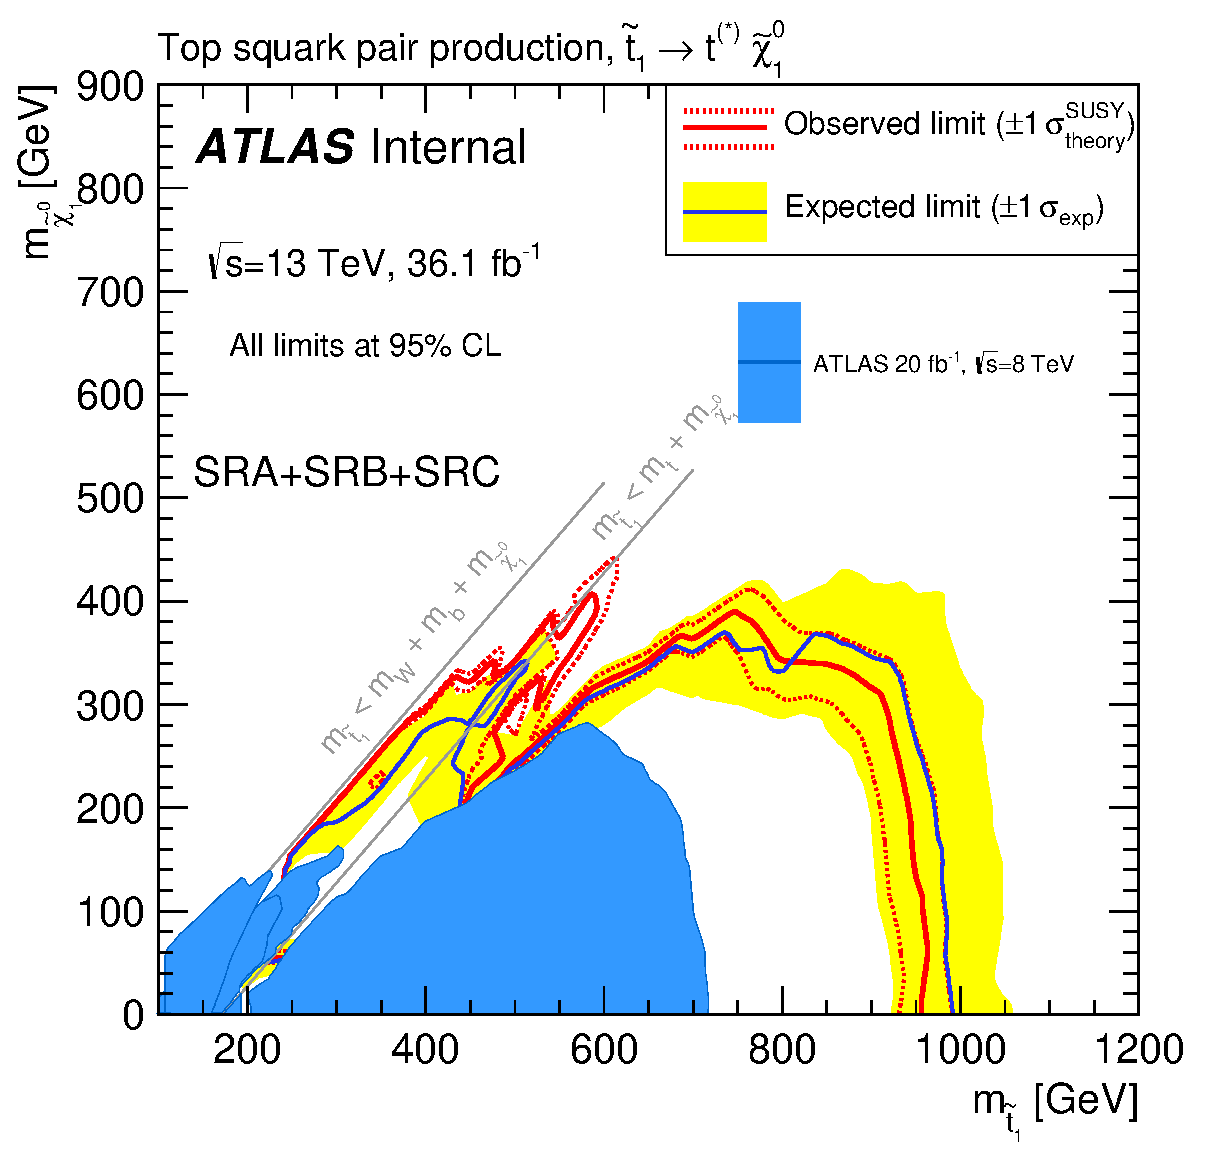
\includegraphics[width=0.85\textwidth]{figures/fit/atlascls_m0m12_wband1_showcms0_StopZL2016_SRABC_Tt_directTTplusbWN_all_Output_fixSigXSecNominal_hypotest__1_harvest_list.eps}
		\caption[95\% confidence limit curves in the stop, neutralino mass parameter space for the compressed stop analysis and the bulk region stop 0L analysis]{
		95\% confidence limit curves in the stop, neutralino mass parameter space for the compressed stop analysis (SRC) and the bulk region stop 0L analysis (SRA+SRB).The solid red (black) line correspond to the 95\% confidence observed (expected) limit curve from all three analysis combined. All regions below the curve has been excluded to 95\% confidence.  The dashed red line is the 95\% confidence limit on stop signal with a $1\sigma$ increase/decrease in signal production cross section.  The shaded yellow region correspond to the $1\sigma$ variation on the expected limit curve.  The variation on the expected limit curve is derived by fitting independent toy experiments and deriving an envelope of confidence limits.  The 8 TeV ATLAS stop search 95\% confidence limits are shown as the shaded blue region in comparison.  The SRA and SRB analyses target high stop masses with large $\Delta m$ and medium amount of $\Delta m$.  Together these two analyses are sensitive to stop masses up $\sim900-1000 \gev$ if the neutralino mass is below $\sim350 \gev$. SRC correspond to the compressed region analysis and adds sensitivity to the $\Delta m = m_{t}$ diagonal region where SRA, SRB and the 8 TeV ATLAS stop searches lack sensitivity.   }
		\label{figure.exclusion.SRABC}
	\end{center}
\end{figure}

\indent Figure \ref{figure.exclusion.SRABCD_dm1} show how the exclusion limit on the stop/neutralino parameter space plane for different the branching fraction of $\stop \rightarrow t+\ninoone$ and $\stop \rightarrow b+\chinoonepm$.  As the $\stop \rightarrow t+\ninoone$ branching fraction decreases, the $\stop \rightarrow b+\chinoonepm$ branching fraction increases with total branching ratio of the two channels adding to one.  Sensitivity from another signal region {\tt SRD} that directly targets the mixed decay channel is combined with the compressed analysis (SRC) and the bulk region analyses (SRA+SRB).  Detailed documentation on the mixed decay analysis can also be found in \cite{stop0Lmoriond}.  Again the compressed analysis is responsible for the exclusion of all stop parameter space along the $\Delta m = m_{t}$ diagonal line when branching fraction to $\stop \rightarrow t+\ninoone$ is high. \\

\begin{figure}[h!]
	\begin{center}
		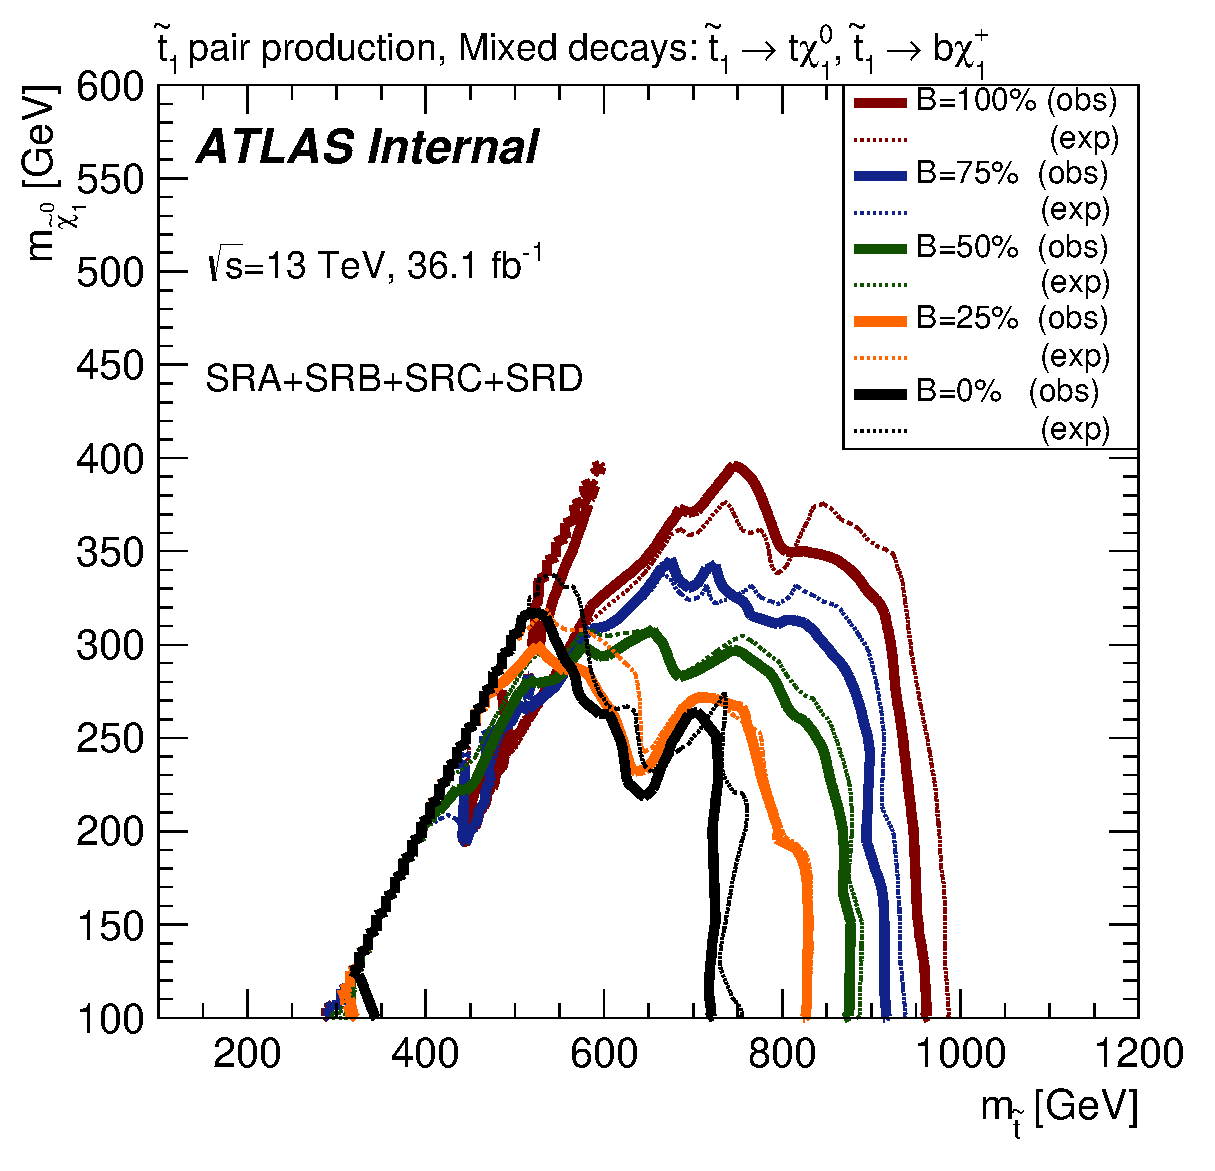
\includegraphics[width=0.85\textwidth]{figures/fit//SRABCD_mixed_dm1.eps}
		\caption[95\% confidence limit curves in the stop, neutralino mass plane for when the stop can decay through two different decay channels: $\stop\ra t\ninoone$
                  and $\stop\ra b\chinoonepm$]{
		95\% confidence limit curves in the stop, neutralino mass plane for when the stop can decay through two different decay channels: $\stop\ra t\ninoone$
                  and $\stop\ra b\chinoonepm\ra b W^{(*)}\ninoone$, with $m(\chinoonepm)-m(\ninoone) = 1 GeV$. 
		 The results are shown for different values of the
                  branching ratio to $\stop\ra t\ninoone$: 0\%, 25\%, 50\%, 75\% and 100\%.  
                  The results are based on a combination of the compressed stop analysis (SRC) targeting $\stop\ra t\ninoone$ with $\Delta m = m_{\stop} - m_{\ninoone} = m_{t}$, the bulk region stop 0 lepton search (SRA+SRB) targeting $\stop\ra t\ninoone$ with $\Delta m >> m_{t}$, and the mixed decay stop search (SRD) targeting stops that decays via both the $\stop\ra t\ninoone$ and $\stop\ra b\chinoonepm$ channels.  The combination take the result from the analysis with the best
                  expected $CL_s$ for the stop, neutralino mass point and the specific decay fraction. 
                   We can see that the compressed analysis SRC adds sensitivity to the $\Delta m = m_t$ line when the branching fraction is mainly to $\stop\ra t\ninoone$.}
		\label{figure.exclusion.SRABCD_dm1}
	\end{center}
\end{figure}